\documentclass[10pt,a4paper,twocolumn]{article}

% ── Packages ──────────────────────────────────────────────────────
\usepackage[utf8]{inputenc}
\usepackage[T1]{fontenc}
\usepackage{lmodern}
\usepackage[margin=1.5cm,top=1.8cm,bottom=1.5cm]{geometry}
\usepackage{booktabs}
\usepackage{amsmath}
\usepackage{hyperref}
\usepackage{xcolor}
\usepackage{enumitem}
\usepackage{titlesec}
\usepackage{array}
\usepackage{graphicx}
\usepackage{float}
\usepackage{caption}
\graphicspath{{figures/}}
\usepackage{tikz}
\usetikzlibrary{arrows.meta,positioning,shapes.geometric,fit,backgrounds,calc}

\hypersetup{colorlinks=true,linkcolor=blue!60!black,urlcolor=blue!60!black}

% IEEE-style centered small-caps headings
\titlespacing*{\section}{0pt}{6pt}{3pt}
\titleformat{\section}{\normalfont\scshape\centering}{\Roman{section}.}{0.5em}{\MakeUppercase}

% Reduce spacing
\setlength{\parskip}{1pt}
\setlength{\parindent}{1em}
\setlength{\columnsep}{0.6cm}
\setlist{nosep,leftmargin=1.2em}

\raggedright
\setlength{\emergencystretch}{1em}
\setlength{\intextsep}{4pt}
\setlength{\textfloatsep}{4pt}
\setlength{\floatsep}{4pt}
\setlength{\abovecaptionskip}{4pt}
\setlength{\belowcaptionskip}{2pt}

% ── Title ─────────────────────────────────────────────────────────
\title{
    \vspace{-1.6cm}
    \textbf{\Large Telekinex: Closed-Loop Brain-to-Robot Control} \\[0.15cm]
    \textbf{\Large via Non-Invasive EEG Decoding} \\[0.2cm]
    \normalsize Kernel \& Dimensional VC Track
    \vspace{-0.3cm}
}
\author{\small
\renewcommand{\arraystretch}{0.9}
\begin{tabular}{@{}>{\centering\arraybackslash}p{0.32\textwidth} >{\centering\arraybackslash}p{0.32\textwidth} >{\centering\arraybackslash}p{0.32\textwidth}@{}}
Joshua~Law & Mourad~Ouazghire & Dmitry~Fadeev\\
\footnotesize TU~Munich & \footnotesize TU~Darmstadt & \footnotesize TU~Munich\\
\scriptsize \nolinkurl{joshua.law@tum.de} & \scriptsize \nolinkurl{mourad.ouazghire@stud.tu-darmstadt.de} & \scriptsize \nolinkurl{dmitry.fadeev@tum.de}\\
\end{tabular}
}

\begin{document}
\date{}
\maketitle
\thispagestyle{empty}
\pagestyle{empty}

\vspace{-0.3cm}
\section{Problem \& Challenge}

As humanoid robots enter factory floors, operators need intuitive ways to direct them through complex tasks---picking, placing, transporting, and navigating cluttered environments. Traditional control interfaces (joysticks, teach pendants, scripted programs) are slow, require line-of-sight, and occupy the operator's hands. Brain-computer interfaces offer a hands-free alternative, but non-invasive EEG is notoriously noisy: decoding motor imagery from a low-density 6-channel headset into reliable, real-time robot commands remains an open challenge. No existing system closes the loop from raw brain signals to a humanoid executing factory tasks.

\section{Target Audience}

\textbf{Primary:} Factory operators and floor supervisors who need to direct humanoid robots through warehouse and manufacturing tasks without putting down their tools or leaving their station.

\textbf{Secondary:} Robotics engineers building human-robot collaboration systems for industrial settings, and BCI researchers seeking an integrated testbed that goes beyond offline classification to closed-loop robotic control.

\section{Solution \& Core Features}

Telekinex lets an operator control a humanoid robot in a factory environment using brain signals and voice commands, with real-time visual feedback.

\begin{itemize}
    \item \textbf{Brain-controlled steering:} A compact neural network (EEGNet, 12.6K params) decodes 5 motor-imagery classes from 6-channel EEG into robot actions---walk, rotate, stop, grab, shift gear---with temporal stabilization for flicker-free control.
    \item \textbf{Voice-commanded task execution:} Natural-language commands (e.g., ``take the box from the conveyor to pallet 2'') are parsed into multi-step autonomous sequences: navigate, grab, navigate, release.
    \item \textbf{Factory simulation:} A Unitree G1 humanoid operates in a MuJoCo factory with shelves, conveyor belt, pallets, and obstacles. Waypoint navigation, obstacle avoidance, and pick-and-place are built in (Fig.~\ref{fig:simulation}).
    \item \textbf{Multimodal fusion:} Voice commands take priority for complex tasks; brain signals provide continuous hands-free directional control; manual keyboard input serves as fallback.
    \item \textbf{Live dashboard:} A web interface displays real-time EEG waveforms, a 2D factory map with robot trail, brain predictions with confidence, command log, and voice input status (Fig.~\ref{fig:dashboard}).
\end{itemize}

\section{Unique Selling Proposition}

Telekinex is the first system to \textbf{close the full loop} from non-invasive EEG to a humanoid robot performing factory tasks---not just classifying signals, but actually steering a simulated robot through pick-and-place and transport workflows. The \textbf{multimodal control layer} (brain + voice + manual) makes it practical: voice handles complex multi-step tasks while brain signals provide continuous hands-free steering, meaning an operator can direct the robot without interrupting their own manual work.

\section{Implementation \& Technology}

The full system architecture is shown in Fig.~\ref{fig:architecture}.

\begin{itemize}
    \item \textbf{ML pipeline:} EEGNet (PyTorch $\to$ ONNX), 0.46\,ms CPU inference. Butterworth bandpass preprocessing, confidence gating + vote buffer + hysteresis for temporal stabilization.
    \item \textbf{Simulation:} MuJoCo physics engine (50\,Hz), Unitree G1 humanoid, custom factory scene with navigable waypoints, collision geometry, and grabbable objects.
    \item \textbf{Backend:} FastAPI server with 10\,Hz WebSocket control loop, gear state machine, regex-based compound voice parser, and sequential action queue for multi-step task execution.
    \item \textbf{Frontend:} Vanilla JS dashboard with Web Speech API, Canvas-rendered EEG chart and 2D factory map, keyboard controls.
\end{itemize}

\section{Results \& Impact}

\begin{itemize}
    \item \textbf{EEG classification accuracy:}\\[2pt]
    \begin{small}
    \begin{tabular}{@{}lccl@{}}
    \toprule
    \textbf{Task} & \textbf{Acc.} & \textbf{Chance} & \textbf{Best class} \\
    \midrule
    Binary (R vs L Fist) & \textbf{63.4\%} & 50\% & --- \\
    5-class              & \textbf{35.2\%} & 20\% & Tongue (F1\,=\,.54) \\
    \bottomrule
    \end{tabular}
    \end{small}\\[1pt]
    Hand-crafted baselines (LR, SVM) at chance level, validating learned temporal features.
    \item \textbf{Sub-millisecond inference} (0.46\,ms), well within the 250\,ms real-time budget.
    \item \textbf{Stable closed-loop control:} Temporal stabilizer yields jitter-free commands at 1--2\,s latency---usable for real humanoid steering.
    \item \textbf{End-to-end voice automation:} Compound commands execute full pick-and-place workflows autonomously.
    \item \textbf{Full system built in 18 hours} by a 3-person team.
\end{itemize}

\vspace{4pt}
\noindent\textbf{Dataset:} 900 EEG recordings (6 subjects, 500\,Hz, 6 channels, 5 motor-imagery classes) from the Kernel Flow dataset.

\vspace{2pt}
\noindent\textit{If we had 24 more hours, we'd connect a live EEG headset and deploy to a physical Unitree G1 on a real factory floor.}

% ══════════════════════════════════════════════════════════════════
% FIGURES (do not count toward page limit)
% ══════════════════════════════════════════════════════════════════
\newpage
\onecolumn

% ── Figure 1: Dashboard ──
\begin{figure}[H]
\centering
\includegraphics[width=\textwidth]{dashboard.png}
\caption{Telekinex Control Dashboard. The interface shows the gear state and brain decode panel (left), a 2D factory floor map with the robot's navigation trail and waypoint markers (center), live 6-channel EEG waveforms (bottom center), command log with brain and voice entries (right), and voice input with microphone toggle (bottom right). The robot is navigating autonomously to the charging station via voice command.}
\label{fig:dashboard}
\end{figure}
\vspace{-1.2cm}
% ── Figure 2: 3D Simulation ──
\begin{figure}[H]
\centering
\includegraphics[width=\textwidth]{simulation.png}
\caption{MuJoCo 3D factory simulation. The Unitree G1 humanoid carries a box retrieved from the work table and walks toward the factory shelves to place it. The scene includes shelves with stored items, pallets, conveyor belt, safety bollards, and floor lane markings.}
\label{fig:simulation}
\end{figure}

% ── Figure 3: Architecture Diagram ──
\begin{center}
\vspace{0.4cm}

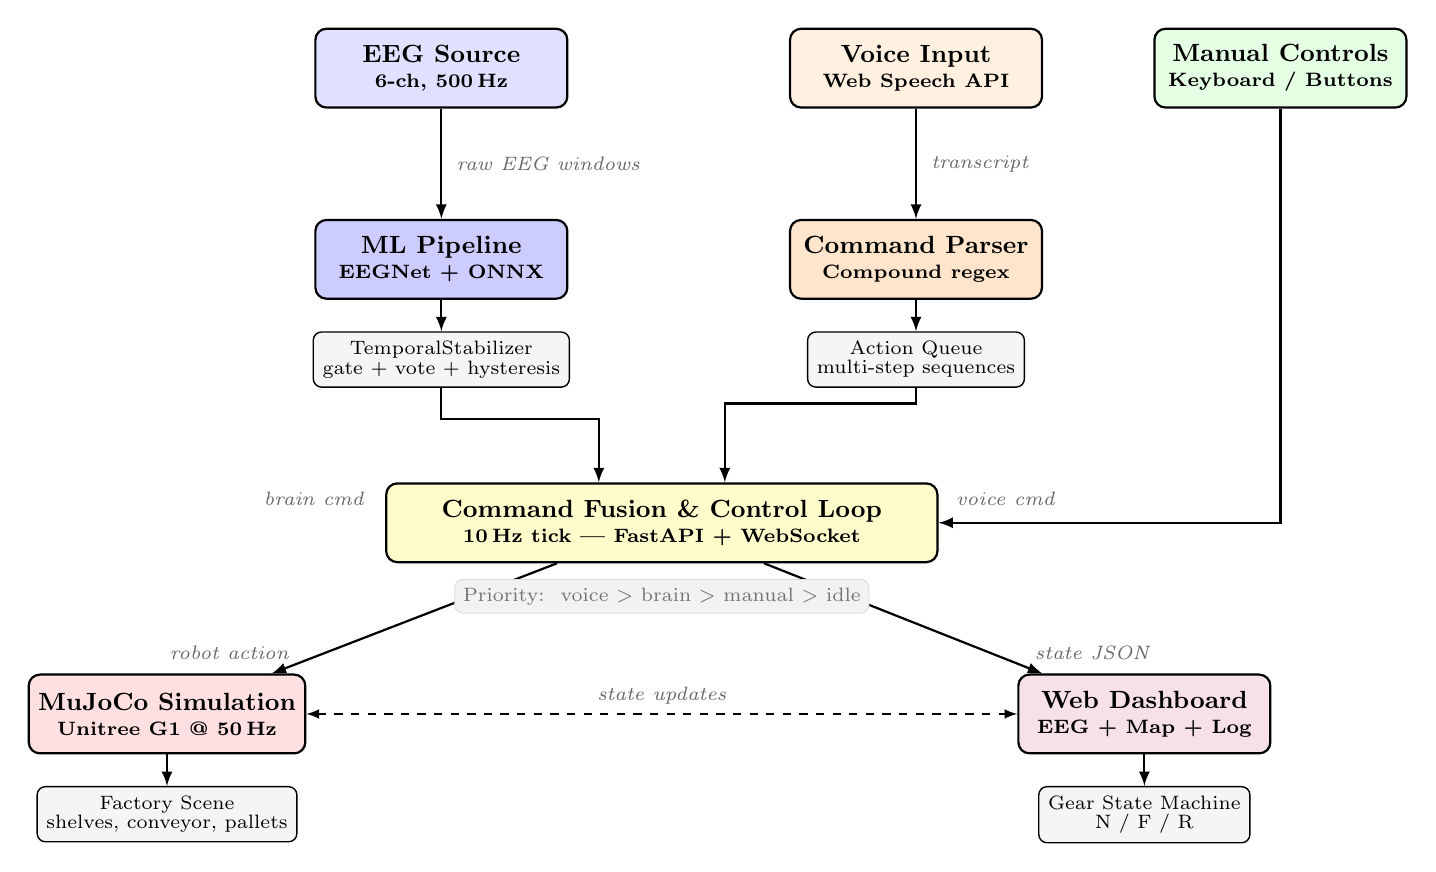
\begin{tikzpicture}[
    node distance=1.2cm and 2.0cm,
    box/.style={draw, rounded corners=4pt, minimum width=3.2cm, minimum height=1cm,
                align=center, font=\small\bfseries, line width=0.8pt},
    smallbox/.style={draw, rounded corners=3pt, minimum width=2.4cm, minimum height=0.7cm,
                     align=center, font=\scriptsize, line width=0.5pt, fill=gray!8},
    arrow/.style={-latex, line width=0.8pt},
    darrow/.style={latex-latex, line width=0.6pt, dashed},
    elabel/.style={font=\scriptsize\itshape, text=black!60},
]

% ── Row 1: Input sources ──
\node[box, fill=blue!12] (eeg) {EEG Source\\[-2pt]\scriptsize 6-ch, 500\,Hz};
\node[box, fill=orange!12, right=2.8cm of eeg] (voice) {Voice Input\\[-2pt]\scriptsize Web Speech API};
\node[box, fill=green!10, right=1.4cm of voice] (manual) {Manual Controls\\[-2pt]\scriptsize Keyboard / Buttons};

% ── Row 2: Processing ──
\node[box, fill=blue!20, below=1.4cm of eeg] (ml) {ML Pipeline\\[-2pt]\scriptsize EEGNet + ONNX};
\node[box, fill=orange!20, below=1.4cm of voice] (parser) {Command Parser\\[-2pt]\scriptsize Compound regex};

% ── Row 2 detail nodes ──
\node[smallbox, below=0.4cm of ml] (stab) {TemporalStabilizer\\[-1pt]\scriptsize gate + vote + hysteresis};
\node[smallbox, below=0.4cm of parser] (queue) {Action Queue\\[-1pt]\scriptsize multi-step sequences};

% ── Row 3: Central orchestrator ──
\node[box, fill=yellow!20, minimum width=7cm, below=1.2cm of stab, xshift=2.8cm] (fusion) {Command Fusion \& Control Loop\\[-2pt]\scriptsize 10\,Hz tick --- FastAPI + WebSocket};

% ── Row 4: Outputs ──
\node[box, fill=red!12, below left=1.4cm and 1cm of fusion] (sim) {MuJoCo Simulation\\[-2pt]\scriptsize Unitree G1 @ 50\,Hz};
\node[box, fill=purple!12, below right=1.4cm and 1cm of fusion] (dash) {Web Dashboard\\[-2pt]\scriptsize EEG + Map + Log};

% ── Sim detail ──
\node[smallbox, below=0.4cm of sim] (factory) {Factory Scene\\[-1pt]\scriptsize shelves, conveyor, pallets};

% ── Gear state machine ──
\node[smallbox, below=0.4cm of dash] (gear) {Gear State Machine\\[-1pt]\scriptsize N / F / R};

% ── Arrows ──
\draw[arrow] (eeg) -- (ml);
\draw[arrow] (voice) -- (parser);
\draw[arrow] (ml) -- (stab);
\draw[arrow] (parser) -- (queue);
\draw[arrow] (stab.south) -- ++(0,-0.4) -| ([xshift=-0.8cm]fusion.north);
\draw[arrow] (queue.south) -- ++(0,-0.2) -| ([xshift=0.8cm]fusion.north);
\draw[arrow] (manual.south) -- (manual.south |- fusion.east) -- (fusion.east);
\draw[arrow] (fusion) -- (sim);
\draw[arrow] (fusion) -- (dash);
\draw[arrow] (sim) -- (factory);
\draw[arrow] (dash) -- (gear);
\draw[darrow] (sim.east) -- (dash.west) node[midway, above, elabel] {state updates};

% ── Edge labels ──
\node[elabel, right=2pt] at ($(eeg.south)!0.5!(ml.north)$) {raw EEG windows};
\node[elabel, right=2pt] at ($(voice.south)!0.5!(parser.north)$) {transcript};
\node[elabel, left=0.15cm of fusion.west, yshift=0.3cm] {\scriptsize brain cmd};
\node[elabel, right=0.1cm of fusion.east, yshift=0.3cm] {\scriptsize voice cmd};
\node[elabel, above left=0.05cm and 0.1cm of sim.north east] {robot action};
\node[elabel, above right=0.05cm and 0.1cm of dash.north west] {state JSON};

% ── Priority annotation ──
\node[rounded corners=3pt, fill=black!5, draw=black!15, line width=0.3pt,
      font=\scriptsize, text=black!55, inner sep=3pt,
      below=0.2cm of fusion] {Priority:\; voice $>$ brain $>$ manual $>$ idle};

\end{tikzpicture}
\captionof{figure}{System architecture. Three input modalities (EEG, voice, manual) are processed through dedicated pipelines and merged by the command fusion layer at 10\,Hz. The fused commands drive the MuJoCo simulation while the web dashboard provides real-time feedback.}
\label{fig:architecture}
\end{center}

\end{document}
